\documentclass{article}
\usepackage{graphicx}
\usepackage{listings}
\usepackage{ctex}
\usepackage{graphicx}
\usepackage[a4paper, body={18cm,22cm}]{geometry}
\usepackage{amsmath,amssymb,amstext,wasysym,enumerate,graphicx}
\usepackage{float,abstract,booktabs,indentfirst,amsmath}
\usepackage{array}
\usepackage{booktabs} %调整表格线与上下内容的间隔
\usepackage{multirow}
\usepackage{diagbox}
\usepackage{indentfirst}
\usepackage{bm}
\usepackage{fancyhdr}




\pagestyle{fancy}

\lhead{\bfseries \normalsize 学号:1952033\quad 姓名:侯雅玥 \quad 组员:廖宏 \\实验名称:集成运算放大电路的应用\quad 课程名称:电子技术实验\quad 专业:微电子科学与工程 } 
\rhead{}

\begin{document}
	\section{\zihao{4} 实验名称:集成运算放大电路的应用(二)}
    \section{\zihao{4} 实验目的}
    \zihao {5} (1)熟悉加法、减法、积分、微分电路的基本工作原理和电路组成形式.\par
               (2)掌握运算电路的设计与实际测量方法.\par
               (3)学会测试各运算电路的工作波形. \par
             
			   \section{\zihao{4} 实验原理}
               (1)加法器\par 
               加法器的输出量反映出多个模拟输入量相加的结果.用运算放大器实现加法运算时,
               可以采用反相输入方式,也可以采用同相输入方式.如图1所示的反相输入加法器,
               是将两个电压 U,和U2同时加到集成运算放大器的反相输入端,显然,它属于多端
               输入的电压并联负反馈电路.在理想情况下,利用虚地的概念,可得到输出电压与输入电压之间的关系为
               \begin{equation*}
                \ U_o=-(\frac{R_f}{R_1}U_{i1}+\frac{R_F}{R_2}U_{i2})
               \end{equation*}
              
            式中,负号是由于反相输入引起的.若$R_1=R_2=R_F$,则上式可变为
            \begin{equation*}
                \ U_o=-(U_{i1}+U_{i2})
               \end{equation*}
如果在输出端再接1级反相器,则可消去式中的负号,这样就可以实现完全符合常规的算术加法运算.\par 
为了提高运算精度,如图1所示的电路中,同相输入端电阻 $R_3$,应满足$R_3=R_1||R_2||R_F$
或增加调零电路.图4-49所示的电路可以扩展到多个输入电压相加的情况,若有几个输入电压相加,
则输出电压与输入电压之间的关系为
\begin{equation*}
    \ U_o=-\sum_{k = 1}^{n}  \frac{R_F}{R_k}U_{ik}
   \end{equation*}
   而$R_P=R_1||R_2||...||R_k||R_F$,扩展后的加法器称为比例加法器,如果电路中取$R_1=R_2=...=R_k=R_F$,
   则有$U_o=-\sum_{k=1}{n}U_{ik}$加法器的输入信号也可以是直流信号.\par 
   \begin{figure}[h]
    %\small
    \centering
    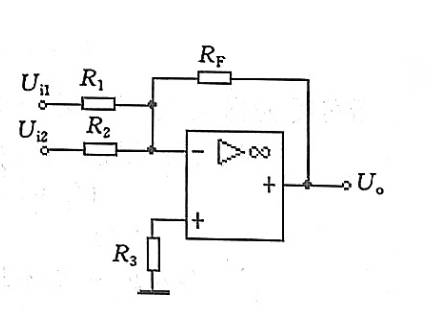
\includegraphics[width=12cm]{H:/电子技术试验/4-14/4-14-1.png}
    \caption{反相加法器} \label{fig:aa}
\end{figure}\par 
   (2)减法器(差动放大器)
   图2是用来实现两个电压 $U_{i1},U_{i2}$相减的电路图. 从结构上看,它是一个反相输入和同相输入相结合的放大器,
   信号电压$U_{i1},U_{i2}$分别通过电阻$R_1,R_2$加在运算放大器的反相和同相输入端$R_F$和$R_1$构成反馈网络.
   当电路参数一定时,由于集成运算放大器的开环电压增益 A.很大,不论 $(U_{i2}-U_{i1})$的大小、
   极性如何,都将引入很强的负反馈,使$U_-=U_+$,电路中存在"虚短"现象,同时两输入端
   引人共模电压,$U_-=U_+=U_{i2}\frac{R_3}{R_3+R_2}$.根据理想运放的两个基本法则,由图2可列出下列方程∶
   \begin{equation*}
    \ \frac{U_{i1}-U_{-}}{R_1}=\frac{U_{-}-U_{o}}{R_F}
   \end{equation*}
   \begin{equation*}
    \ \frac{U_{i2}-U_{+}}{R_2}=\frac{U_+}{R_3}
   \end{equation*}

   从而可得输出电压
   \begin{equation*}
  \  U_o=(\frac{R_1+R_F}{R_1})(\frac{R_3}{R_2+R_3})U_{i2}-\frac{R_F}{R_1}U_{i1}
\end{equation*}
   当电阻值满足$R_F||R_1=R_2||R_3$的关系时,输出电压可简化为
   \begin{equation*}
    \  U_o=\frac{R_F}{R_1}(U_{i2}-U_{i1})
  \end{equation*}
  
     输入电阻为
   \begin{equation*}
    \  R_1=R_1+R_2=2R_1
  \end{equation*}
差模增益为
\begin{equation*}
    \  A_{ud}=\frac{U_o}{U_{i2}-U_{i1}}=\frac{R_F}{R_1}=\frac{R_3}{R_2}
  \end{equation*}
   即输出电压U。与两个输入电压之差$U_{i2}-U_{i1}$成比例.当取${R_F}={R_1}$时$U_o=U_{i2}-U_{i1}$可实现减法运算.
   这种电路常用于将差动输出转换为单端输出,放大具有强烈共模干扰的微弱信号,
            或用于传感器、测量仪器的前置放大.要提高运算精度,一方面要严格选配电阻,
            另一方面要采用高共模抑制比的集成运算放大器.
             \begin{figure}[h]
                %\small
                \centering
                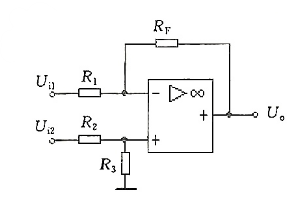
\includegraphics[width=12cm]{H:/电子技术试验/4-14/4-14-2.png}
                \caption{反相加法器} \label{fig:aa}
            \end{figure}\par 

         
            (3)积分器
            积分电路是模拟计算机中的基本单元,利用它可以实现微分方程的模拟,它同时也是控制和测量系统中的重要单元,
            利用它的充放电过程可以实现延时、定时以及产生各种波形.集成运算放大器的基本积分电路
            如图3所示.它和反相比例放大器的不同之处在于它是用电容C来代替反馈电阻R利用集成运算放大器,
            电容C两端电压增长时流过它的电流基本维持稳定,从而可以实现比较理想的积分运算.   
            由于$i_1=\frac{u_i}{R_1}=-i_c$    
            \begin{equation*}
                \  u_o(t)=-\frac{1}{C}\int_{0}^{t}i_c  \, dt=-\frac{1}{R_1C}\int_{0}^{t} u_i\, dt 
              \end{equation*}

            
上式表明输出电压与输入电压成积分关系,式中负号表示输出电压与输入电压在相位上是相反的.
为了减小输入偏置电流的影响,同相端平衡电阻$R_p=R_1$.
当输人信号是幅度为$U_m$的阶跃电压时,
\begin{equation*}
    \  u_o(t)=-\frac{1}{R_1C}\int_{0}^{t} U_m\, dt=-\frac{U_mt}{R_1C} 
  \end{equation*}
上式说明,输出电压与输入电压相位相反,且输出电压(z)随时间的增长线性下降,
直到放大器出现饱和.当 t=RC时,$u_o(t)=-U_m$
若输入是方波,则输出电压为锯齿波,且两者相位相反.
实际中,为了限制电路的低频增益,减小失调电压的影响,电路如图4所示
\begin{figure}[h]
	\begin{minipage}[t]{0.5\linewidth} % 如果一行放2个图,用0.5,如果3个图,用0.33  
	  \centering   
	  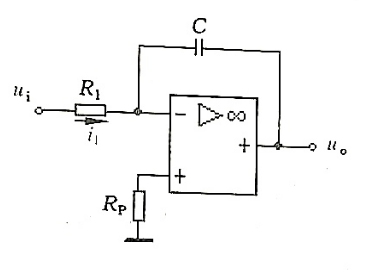
\includegraphics[width=3in]{H:/电子技术试验/4-14/4-14-3.png}   
	  \caption{积分器原理}   
	  \label{fig:side:a}   
	\end{minipage}%   
	\begin{minipage}[t]{0.5\linewidth}   
	  \centering   
	  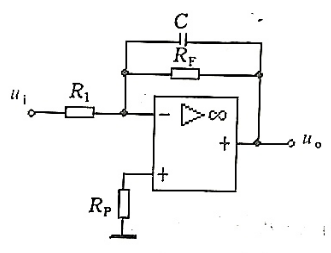
\includegraphics[width=3in]{H:/电子技术试验/4-14/4-14-4.png}   
	  \caption{积分器实验}   
	  \label{fig:side:b}   
	\end{minipage}   
  \end{figure}
  \par 
  (4)微分器\par 
  微分运算是积分运算的逆运算.从电路形式上看,将图3中电阻与电容的位置对调一下,即可得到图5所示的微分电路.
 由于
 \begin{equation*}
    \  i_i=C\frac{du_i}{dt} 
  \end{equation*}

  \begin{equation*}
    \  i_1=i_C 
  \end{equation*}
  \begin{equation*}
    \  u_o(t)=-i_cR_F=-R_FC \frac{du_i}{dt}
  \end{equation*}

  即输出电压是输入电压的微分,$R_P=R_F$从而可实现微分运算.
 
利用微分电路可以实现波形变换,如将矩形波变换成为尖脉冲,若输入信号为对称三角波,则输出电压为对称的方波.
  
  
  \begin{figure}[h]
	\begin{minipage}[t]{0.5\linewidth} % 如果一行放2个图,用0.5,如果3个图,用0.33  
	  \centering   
	  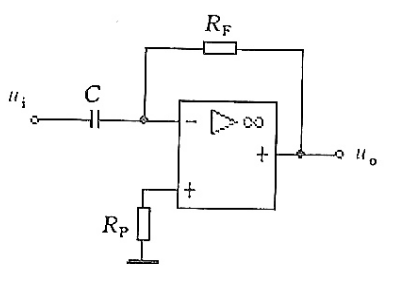
\includegraphics[width=3in]{H:/电子技术试验/4-14/4-14-5.png}   
	  \caption{微分器原理}   
	  \label{fig:side:a}   
	\end{minipage}%   
	\begin{minipage}[t]{0.5\linewidth}   
	  \centering   
	  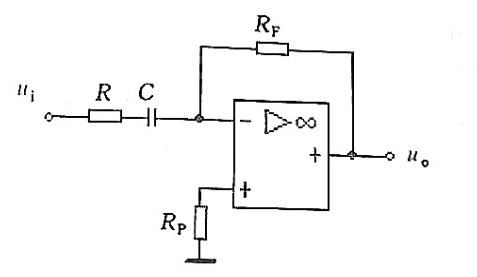
\includegraphics[width=3in]{H:/电子技术试验/4-14/4-14-6.png}   
	  \caption{微分器实验}   
	  \label{fig:side:b}   
	\end{minipage}   
  \end{figure}

\section{\zihao{4} 实验电路}
\begin{figure}[h]
	\begin{minipage}[t]{0.5\linewidth} % 如果一行放2个图,用0.5,如果3个图,用0.33  
	  \centering   
	  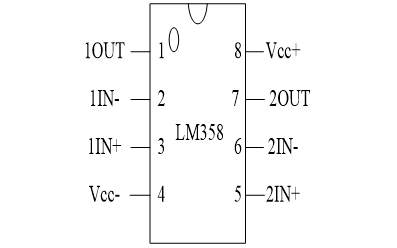
\includegraphics[width=3in]{H:/电子技术试验/4-14/4-14-7.png}   
	  \caption{加法器}   
	  \label{fig:side:a}   
	\end{minipage}%   
	\begin{minipage}[t]{0.5\linewidth}   
	  \centering   
	  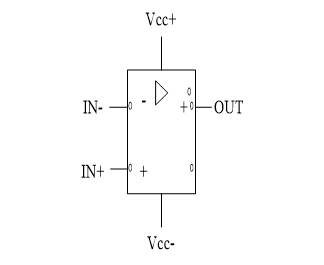
\includegraphics[width=3in]{H:/电子技术试验/4-14/4-14-8.png}   
	  \caption{减法器}   
	  \label{fig:side:b}   
	\end{minipage}   
  \end{figure}
\begin{figure}[h]
	\begin{minipage}[t]{0.5\linewidth} % 如果一行放2个图,用0.5,如果3个图,用0.33  
	  \centering   
	  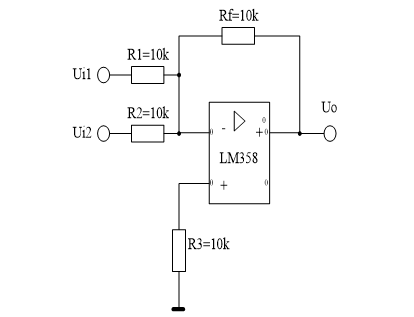
\includegraphics[width=3in]{H:/电子技术试验/4-14/4-14-9.png}   
	  \caption{加法器}   
	  \label{fig:side:a}   
	\end{minipage}%   
	\begin{minipage}[t]{0.5\linewidth}   
	  \centering   
	  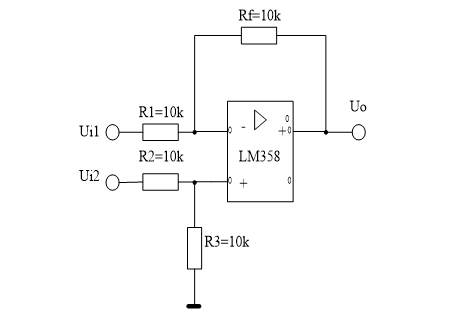
\includegraphics[width=3in]{H:/电子技术试验/4-14/4-14-10.png}   
	  \caption{减法器}   
	  \label{fig:side:b}   
	\end{minipage}   
  \end{figure}
  \begin{figure}[h]
	\begin{minipage}[t]{0.5\linewidth} % 如果一行放2个图,用0.5,如果3个图,用0.33  
	  \centering   
	  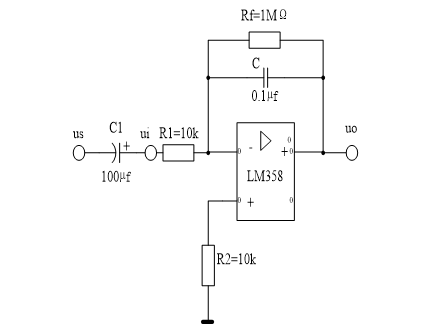
\includegraphics[width=3in]{H:/电子技术试验/4-14/4-14-11.png}   
	  \caption{积分器}   
	  \label{fig:side:a}   
	\end{minipage}%   
	\begin{minipage}[t]{0.5\linewidth}   
	  \centering   
	  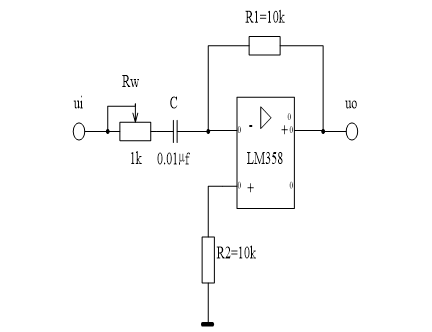
\includegraphics[width=3in]{H:/电子技术试验/4-14/4-14-12.png}   
	  \caption{微分器}   
	  \label{fig:side:b}   
	\end{minipage}   
  \end{figure}

\section{\zihao{4} 实验内容及步骤}
  \subsection{加法器}
  (1)按图9连接好线路,检查无误后接入士12V电源.\par
  (2)在输入端输入不同数值的直流信号,当 $R_1,R_2$为不同值时,测出所对应的输出电压.记录数据,根据电路元件参数值进行理论计算,将计算结果填入同一表中,并与测量值相比较。
  \par
  \subsection{减法器}
 (1)按图10连接好线路,检查无误后接入士12V电源。\par
 (2)在输入端输入不同数值的直流信号,当 和为不同值时,测出所对应的输出电压.记录数据,根据电路元件参数值进行理论计算,将计算结果填入同一表中,并与测量值相比较。
 \par
 \subsection{积分器}

 (1)参照图11接好线路,检查无误后通电。\par
 (2)分别输入频率 f=1kHz,Uip-p=1.5V的方波信号、正弦波信号,三角波信号,用示波器同时观测和记录、的波形、幅度及相位。
 \par
 \subsection{微分器}
 (1)参照图12接好线路,检查无误后通电。
 (2)输入频率 f=500Hz,Uip-p=1.5V的三角波信号,调节使输出的方波不出现过冲和塌顶现象(临界补偿),观测和记录、的波形、幅度及相位。再分别输入同频同幅的方波信号、正弦波信号用示波器同时观测和记录、的波形、幅度及相位。最后记录的实际阻值。




\section{\zihao{4} 数据及误差处理}
\subsection{加法器}
\begin{table}[h]
    \centering  
    \begin{tabular}{c|c|c|c}
        \hline
            $U_{i1}(V)$      & 1    & 2    & 3  \\ \hline
            $U_{i2}(V)$       &   3        & 2        &1        \\ \hline
            $U_{0}(V)$(理论值)  &   -4        &-4         &-4      \\ \hline
            $U_{0}(V)$(实验值) &-4.01&-4.02&-4.02  \\ \hline
            $ \delta(u_o) $ &0.2\%&0.4\%&0.4\% \\ \hline
    \end{tabular}
  
    \caption{加法器数据表}\label{SIGN}
    \end{table}
      \subsection{减法器}
    \begin{table}[h]
        \centering  
        \begin{tabular}{c|c|c|c}
            \hline
                $U_{i1}(V)$      & 1    & 2   & 3  \\ \hline
                $U_{i2}(V)$       &   3        & 2        &1        \\ \hline
                $U_{0}(V)$(理论值)  &   2        &0         &-2      \\ \hline
                $U_{0}(V)$(实验值) &2.00&0.01&-2.00  \\ \hline
                $ \delta(u_o) $ &0&0&0 \\ \hline
        \end{tabular}
        \caption{减法器数据表}\label{SIGN}
        \end{table} 
        \newpage
         \subsection{积分器}    
          \begin{figure}[h]
              \begin{minipage}[t]{0.5\linewidth} % 如果一行放2个图,用0.5,如果3个图,用0.33  
                \centering   
                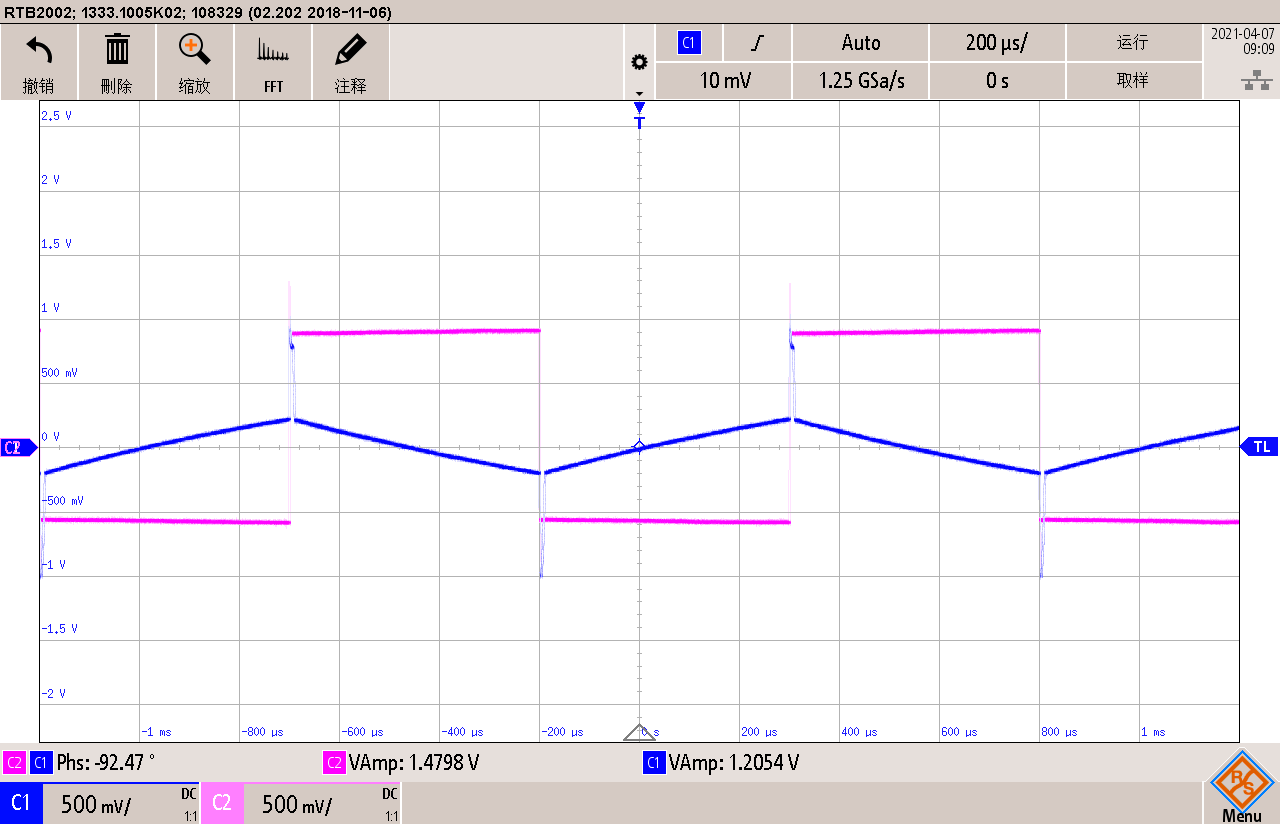
\includegraphics[width=3in]{H:/电子技术试验/4-14/4-14-13.png}   
                \caption{方波输出}   
                \label{fig:side:a}   
              \end{minipage}%   
              \begin{minipage}[t]{0.5\linewidth}   
                \centering   
                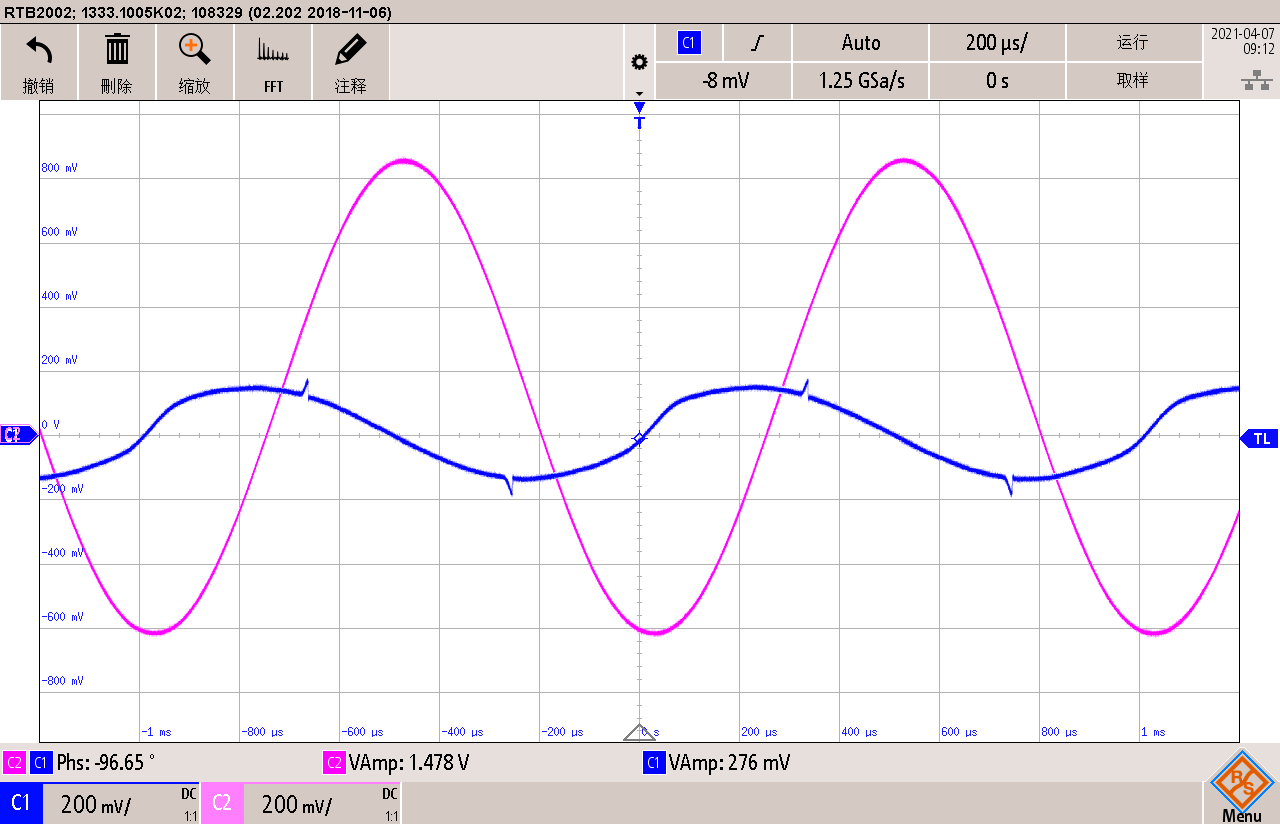
\includegraphics[width=3in]{H:/电子技术试验/4-14/4-14-14.png}   
                \caption{正弦波输入}   
                \label{fig:side:b}   
              \end{minipage}   
              \end{figure}
              \begin{figure}[h]
                %\small
                \centering
                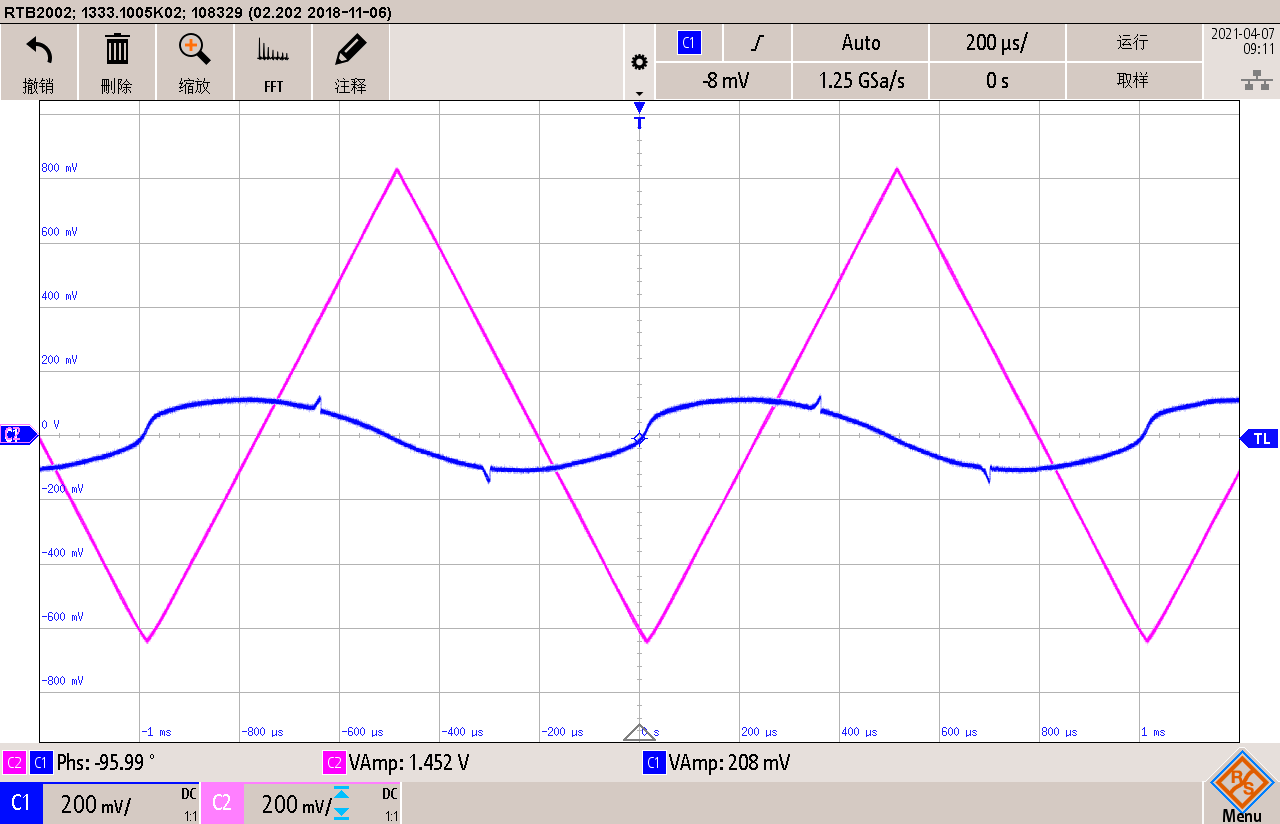
\includegraphics[width=3in]{H:/电子技术试验/4-14/4-14-15.png}
                \caption{三角波输入} \label{fig:aa}
            \end{figure}
        \begin{table}[h]
            \centering  
            \begin{tabular}{c|c|c|c}
                \hline
                   幅度     & 1.205V    & 0.276V   & 0.208V  \\ \hline
                  相位(理论值) &   -90.0       & -90.0        &-90.0        \\ \hline
                  相位(实验值) &  -92.5        &-96.7         &-97.0      \\ \hline
                    $ \delta(Phase) $ &2.7\%&7.4\%&7.8\% \\ \hline
            \end{tabular}
          
            \caption{积分器数据表}\label{SIGN}
            \end{table}  
            \newpage


            \subsection{微分器}
       
            \begin{figure}[h]
              \begin{minipage}[t]{0.5\linewidth} % 如果一行放2个图,用0.5,如果3个图,用0.33  
                \centering   
                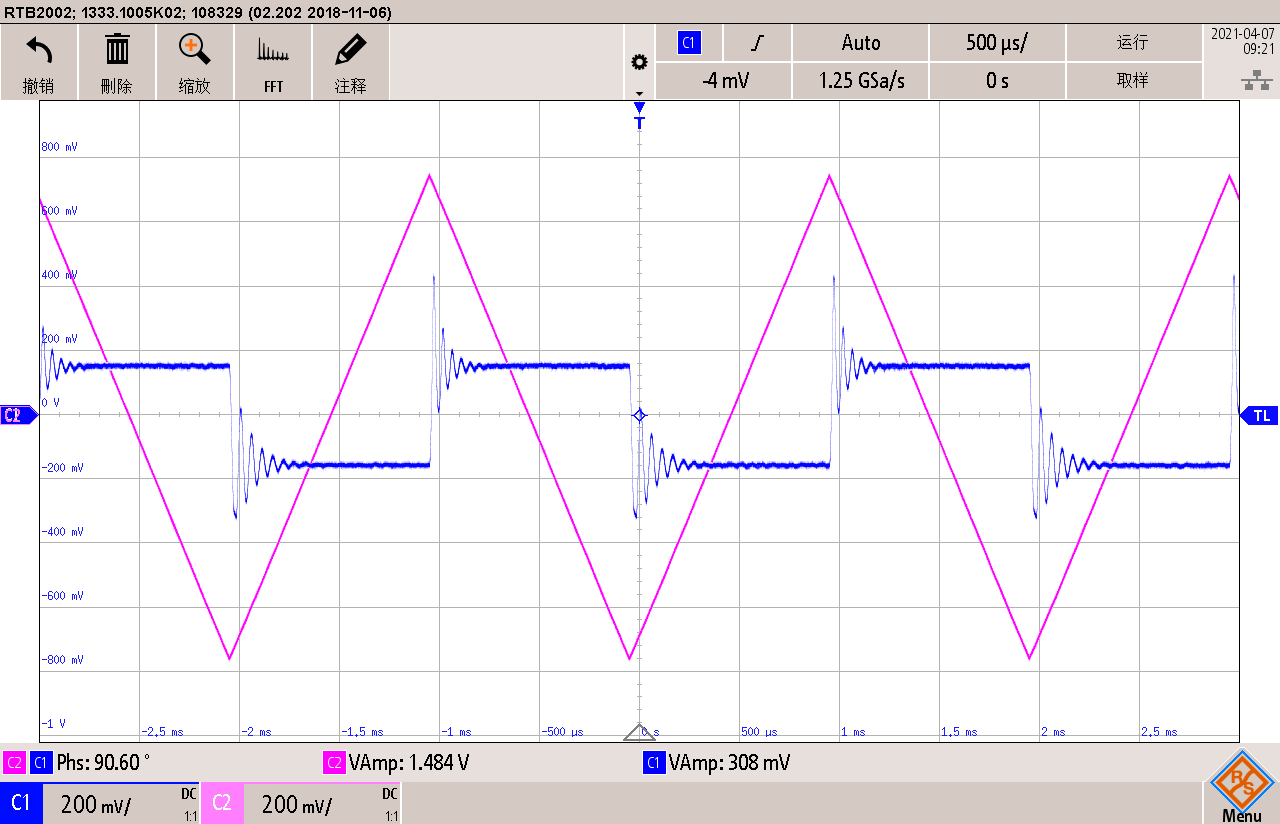
\includegraphics[width=3in]{H:/电子技术试验/4-14/4-14-16.png}   
                \caption{过冲现象}   
                \label{fig:side:a}   
              \end{minipage}%   
              \begin{minipage}[t]{0.5\linewidth}   
                \centering   
                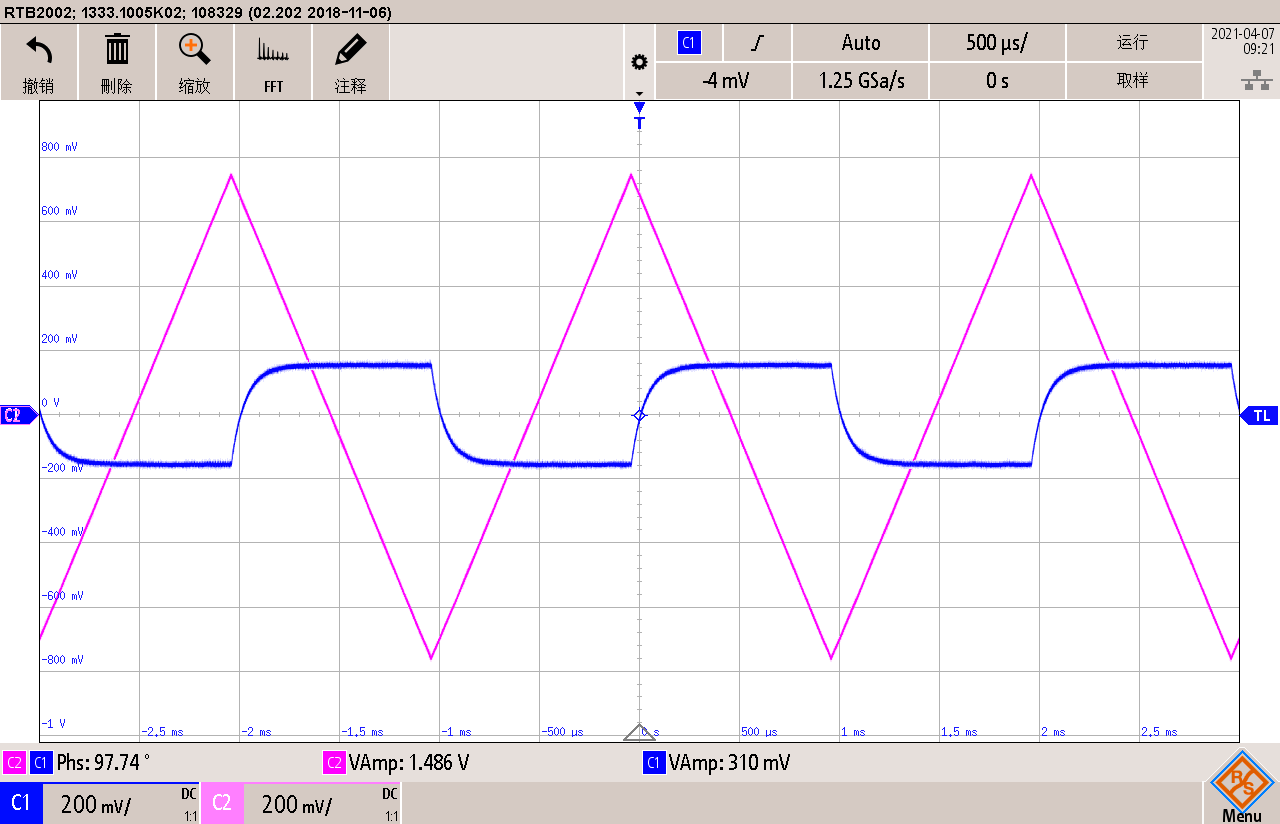
\includegraphics[width=3in]{H:/电子技术试验/4-14/4-14-17.png}   
                \caption{塌陷现象}   
                \label{fig:side:b}   
              \end{minipage}   
              \end{figure}
              \begin{figure}[h]
                %\small
                \centering
                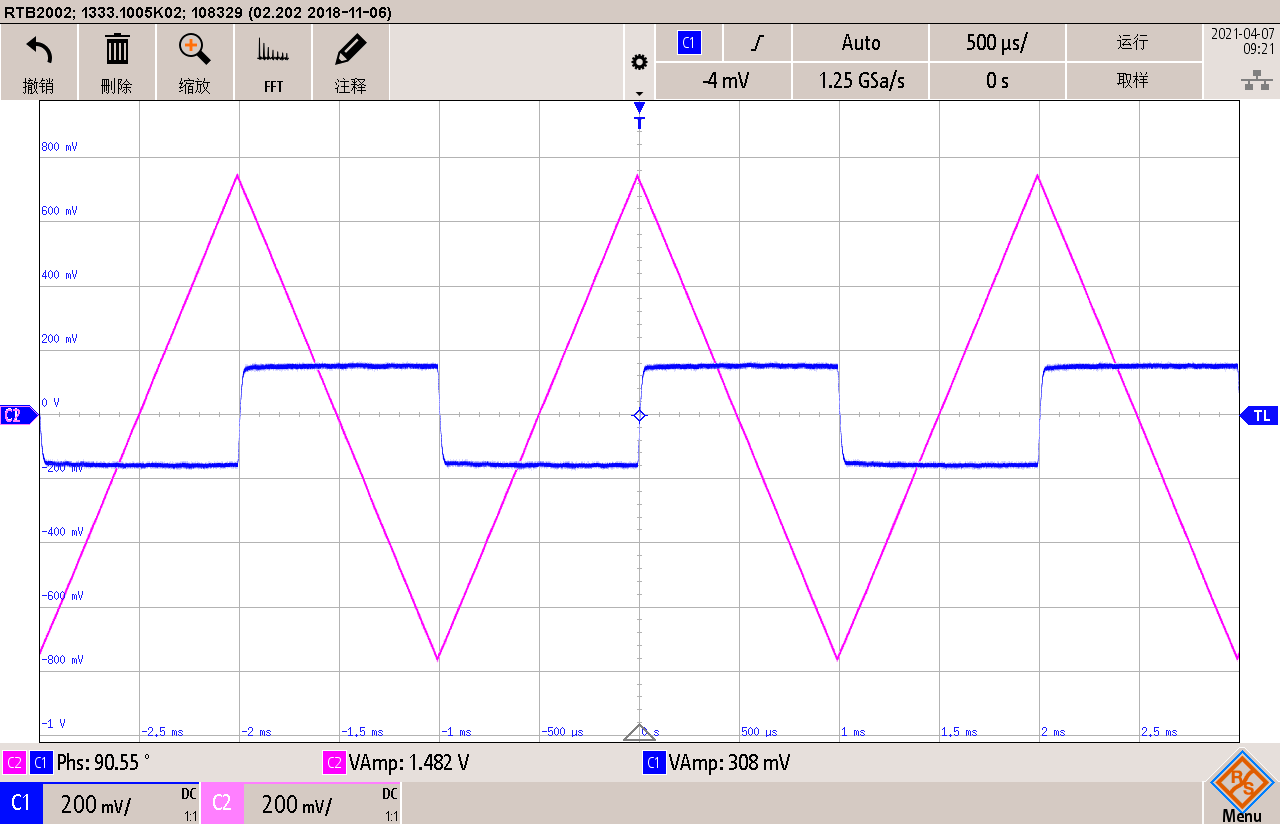
\includegraphics[width=3in]{H:/电子技术试验/4-14/4-14-18.png}
                \caption{实验值} \label{fig:aa}
            \end{figure}

            \begin{figure}[h]
              \begin{minipage}[t]{0.5\linewidth} % 如果一行放2个图,用0.5,如果3个图,用0.33  
                \centering   
                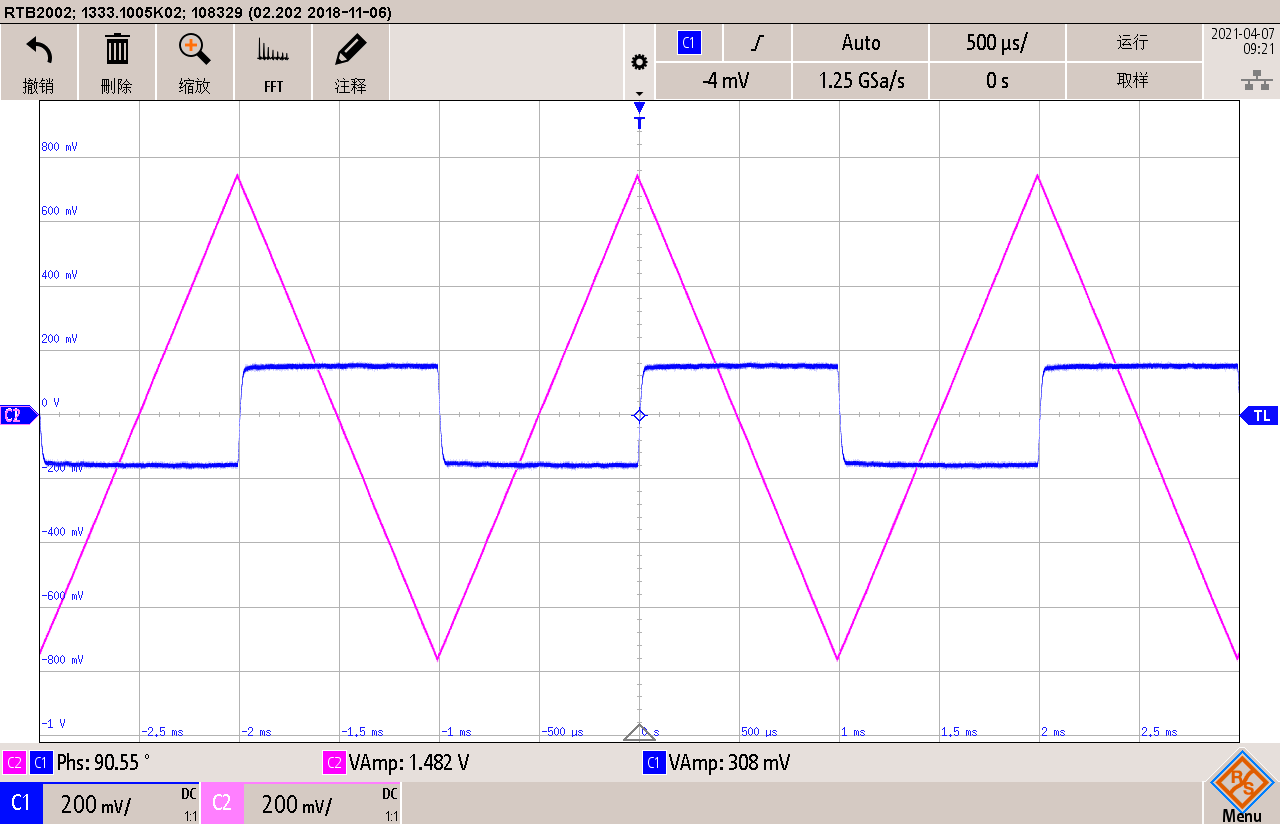
\includegraphics[width=3in]{H:/电子技术试验/4-14/4-14-19.png}   
                \caption{方波输出}   
                \label{fig:side:a}   
              \end{minipage}%   
              \begin{minipage}[t]{0.5\linewidth}   
                \centering   
                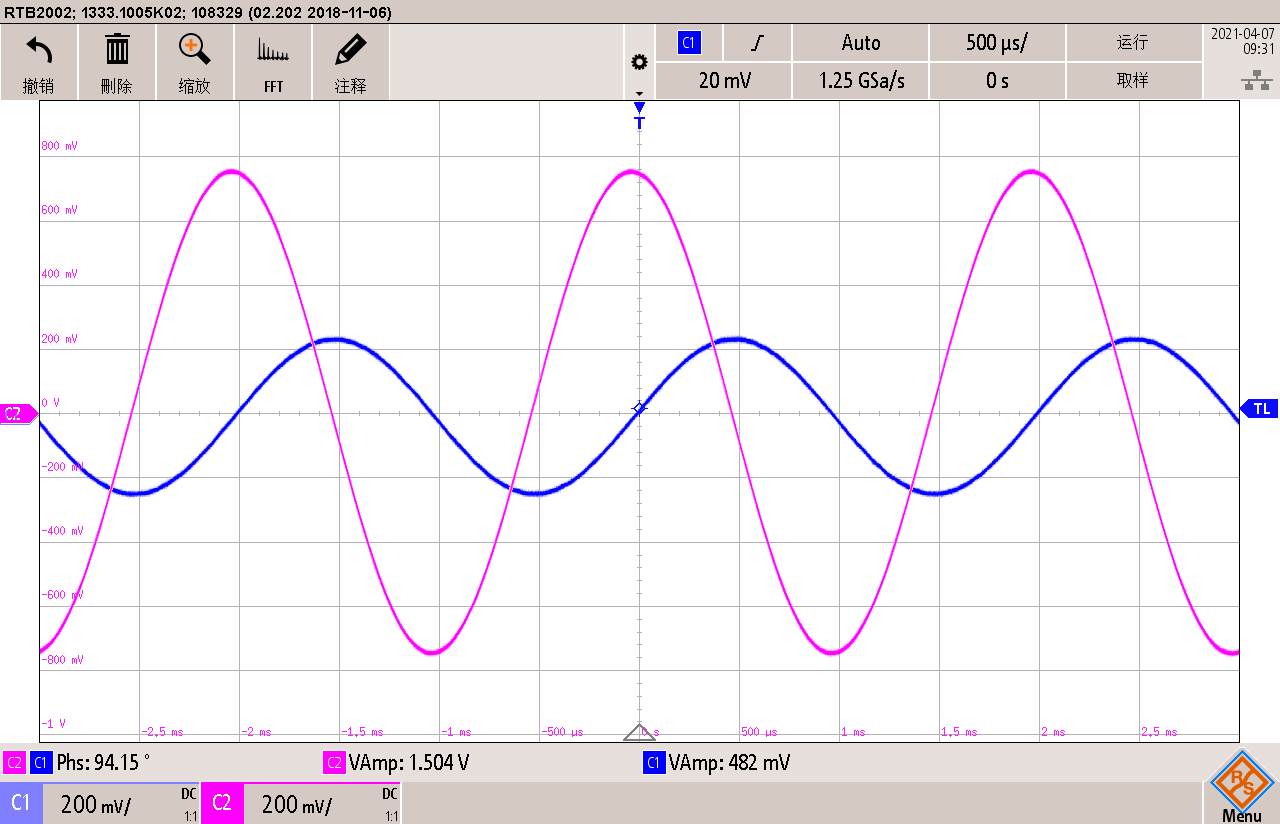
\includegraphics[width=3in]{H:/电子技术试验/4-14/4-14-20.png}   
                \caption{正弦波输入}   
                \label{fig:side:b}   
              \end{minipage}   
              \end{figure}
              \begin{figure}[h]
                %\small
                \centering
                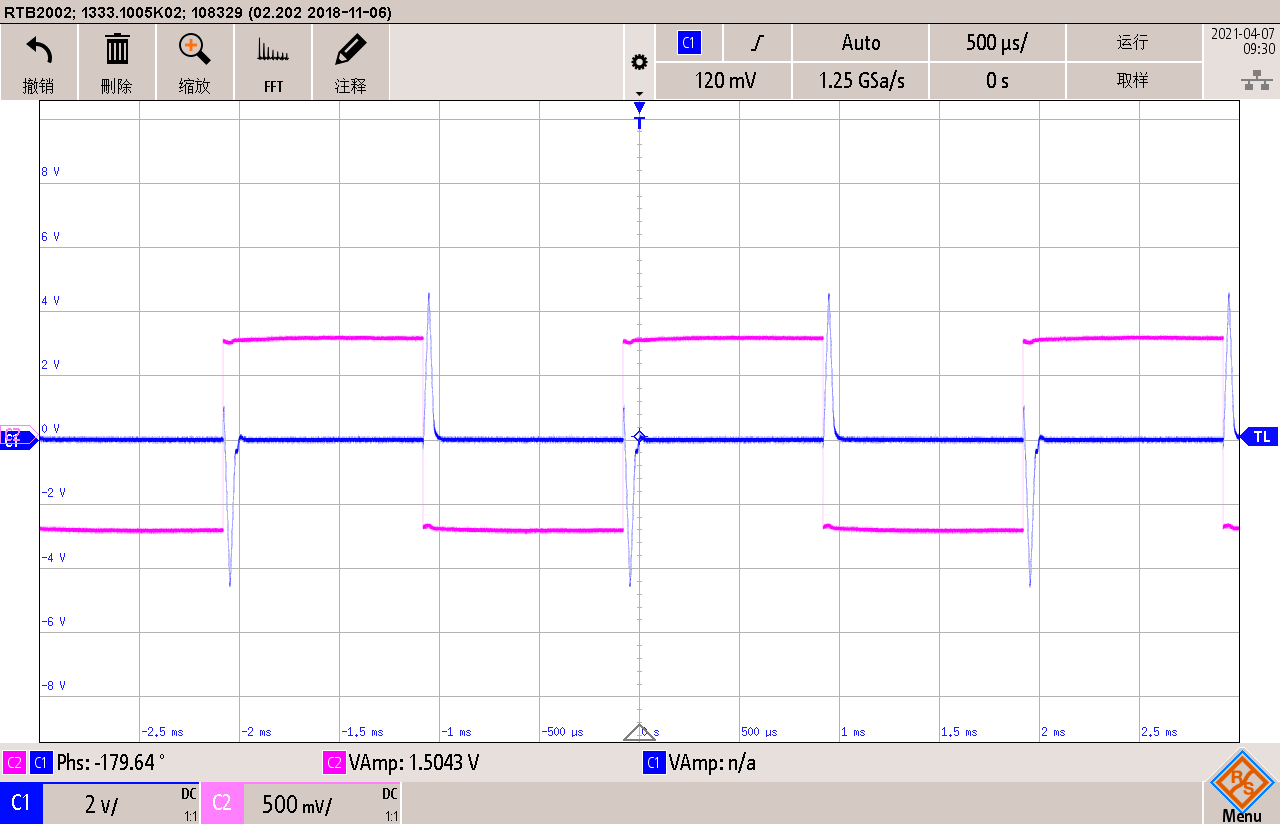
\includegraphics[width=3in]{H:/电子技术试验/4-14/4-14-21.png}
                \caption{三角波输入} \label{fig:aa}
            \end{figure}

          
            \begin{table}[h]
                \centering  
                \begin{tabular}{c|c|c|c}
                    \hline
                       幅度     & 激冲电压    & 0.482V   & 0.308V  \\ \hline
                      相位(理论值) &   -180.0       & 90.0        &90.0        \\ \hline
                      相位(实验值) &  -179.6       &94.1         &90.6      \\ \hline
                        $ \delta(Phase) $ &0.2\%&4.5\%&0.6\% \\ \hline
                \end{tabular}
              
                \caption{微分器数据表}\label{SIGN}
                \end{table}
                \par
                测得$R_W=1.24k\Omega$
              \newpage
	\section{\zihao{4} 实验设备和器材}
	(1)双踪示波器             \qquad \qquad \qquad \qquad \qquad  \qquad           1台\par
	(2)函数信号发生器          \qquad  \qquad \qquad \qquad       \qquad           1台\par
	(3)直流稳压电源             \qquad \quad \qquad \qquad \qquad \qquad           1台\par
	(4)模拟电路实验箱            \qquad  \qquad \qquad \qquad\qquad                1台\par
	(5)万用表                   \qquad  \qquad \qquad \qquad \qquad \qquad \qquad  1只\par
	(6)集成芯片LM358、电阻器、电容器  \quad                                        若干

\section{结论}
(1)加法器\par
加法器,是将两个电压 U,和U2同时加到集成运算放大器的反相输入端,显然,它属于多端
输入的电压并联负反馈电路.在理想情况下,利用虚地的概念,可得到输出电压与输入电压之间的关系为
\begin{equation*}
 \ U_o=-(\frac{R_f}{R_1}U_{i1}+\frac{R_F}{R_2}U_{i2})
\end{equation*}
\par
(2)减法器(差动放大器)
减法器用来实现两个电压和相减的电路图。从结构上看,它是一个反相输人和同相输入相结合的放大器,信号电压和分别通过电阻,加在运算放大器的反相和同相输入端,电阻,构成反馈网络。当电路参数一定时,由于集成运算放大器的开环电压增益很大,电路中也存在"虚短"现象,同时两输入端引入共模电压,最终得到输出电压:
当电阻值满足$R_F||R_1=R_2||R_3$的关系时,输出电压可简化为
\begin{equation*}
 \  U_o=\frac{R_F}{R_1}(U_{i2}-U_{i1})
\end{equation*}
即输出电压与两个输入电压之差$U_{i2}-U_{i1}$成比例.当取${R_F}={R_1}$时$U_o=U_{i2}-U_{i1}$可实现减法运算.

\par
(3)积分器\par
积分电路是模拟计算机中的基本单元,利用它可以实现微分方程的模拟,它同时也是控制和测量系统中的重要单元,利用它的充放电过程可以实现延时、定时以及产生各种波形。它和反相比例放大器的不同之处在于它是用电容C来代替反馈电阻,利用集成运算放大器,电容C两端电压增长时流过它的电流基本维持稳定,从而可以实现比较理想的积分运算。
当输入不同种类的信号时,输出信号也有所不同;
输入方波信号:输出线性信号,相位差为-90
输入正弦波信号:输出余弦波信号,相位差为-90
输入三角波信号:输出类二次函数信号,相位差为-90
\par

(4)微分器\par
微分运算是积分运算的逆运算。从电路形式上看,将积分电路中电阻与电容 C的位置对调一下,即可得到微分电路。
当输入不同种类的信号时,输出信号也有所不同;
输入方波信号:输出脉冲信号,相位差为-180
输入正弦波信号:输出余弦波信号,相位差为90
输入对称三角波信号:输出对称方波信号,相位差为90
\par

\section{思考题}
(1)在积分电路中,电阻起什么作用?\par
电阻保证电路中放大器输入两端电阻大小基本相同,保证电路输入电压可控。
\par
(2)在反相加法器的输出电压中,各相加项的比例系数仅与和输入回路的输入电阻之比有关,而与其他输入端的电阻及运算放大器的参数无关,以上结论在什么条件下才成立?为什么? 反相加法器能否实现减法运算?如何实现?\par
以上条件是理想假设,只有输入端电流完全虚短,电压完全虚断时可以实现。反相加法器可以实现减法运算,即在加法器的基础上加上可控反相器。
\par
(3)如果实际运算放大器不符合理想运算放大器条件,会出现什么问题?如要求

各元件参数应如何确定?\par
答:如果实际运算放大器不符合理想运算放大器条件,则通过“虚短”“虚断”得到的理论数值会与实验数据不相符。如要求,则可以通过公式:
$U_o=\frac{R_F}{R_1}U_{i1}-\frac{R_F}{R_2}U_{i2}$
来确定各项的数值
\par
(4)为了不损坏集成块,实验中应注意什么问题?\par
为了不损坏集成块,集成运算放大器实验中必须注意以下三个问题,不要接错电源的正负极;输入信号的幅值要在运算放大器允许的范围之内。
\end{document}

